\documentclass[man, noextraspace, floatsintext]{apa6}\usepackage[]{graphicx}\usepackage[]{color}
%% maxwidth is the original width if it is less than linewidth
%% otherwise use linewidth (to make sure the graphics do not exceed the margin)
\makeatletter
\def\maxwidth{ %
  \ifdim\Gin@nat@width>\linewidth
    \linewidth
  \else
    \Gin@nat@width
  \fi
}
\makeatother

\definecolor{fgcolor}{rgb}{0.345, 0.345, 0.345}
\newcommand{\hlnum}[1]{\textcolor[rgb]{0.686,0.059,0.569}{#1}}%
\newcommand{\hlstr}[1]{\textcolor[rgb]{0.192,0.494,0.8}{#1}}%
\newcommand{\hlcom}[1]{\textcolor[rgb]{0.678,0.584,0.686}{\textit{#1}}}%
\newcommand{\hlopt}[1]{\textcolor[rgb]{0,0,0}{#1}}%
\newcommand{\hlstd}[1]{\textcolor[rgb]{0.345,0.345,0.345}{#1}}%
\newcommand{\hlkwa}[1]{\textcolor[rgb]{0.161,0.373,0.58}{\textbf{#1}}}%
\newcommand{\hlkwb}[1]{\textcolor[rgb]{0.69,0.353,0.396}{#1}}%
\newcommand{\hlkwc}[1]{\textcolor[rgb]{0.333,0.667,0.333}{#1}}%
\newcommand{\hlkwd}[1]{\textcolor[rgb]{0.737,0.353,0.396}{\textbf{#1}}}%

\usepackage{framed}
\makeatletter
\newenvironment{kframe}{%
 \def\at@end@of@kframe{}%
 \ifinner\ifhmode%
  \def\at@end@of@kframe{\end{minipage}}%
  \begin{minipage}{\columnwidth}%
 \fi\fi%
 \def\FrameCommand##1{\hskip\@totalleftmargin \hskip-\fboxsep
 \colorbox{shadecolor}{##1}\hskip-\fboxsep
     % There is no \\@totalrightmargin, so:
     \hskip-\linewidth \hskip-\@totalleftmargin \hskip\columnwidth}%
 \MakeFramed {\advance\hsize-\width
   \@totalleftmargin\z@ \linewidth\hsize
   \@setminipage}}%
 {\par\unskip\endMakeFramed%
 \at@end@of@kframe}
\makeatother

\definecolor{shadecolor}{rgb}{.97, .97, .97}
\definecolor{messagecolor}{rgb}{0, 0, 0}
\definecolor{warningcolor}{rgb}{1, 0, 1}
\definecolor{errorcolor}{rgb}{1, 0, 0}
\newenvironment{knitrout}{}{} % an empty environment to be redefined in TeX

\usepackage{alltt}
\newcommand{\bibfile}{C:/Users/jep2963/Documents/Bibliography/Behavioral_observation-APP}  

\usepackage[natbibapa]{apacite}
\newcommand{\citetal}[1]{\shortcites{#1}\citet{#1}}

\raggedbottom

\usepackage{amssymb}
\usepackage{amsmath}
\usepackage{amsthm}
\newtheorem{lemma}{Lemma}

\usepackage{graphicx}

\usepackage{fixltx2e}
\usepackage{subcaption}
\usepackage{float}

\usepackage{array}
\usepackage{multirow}
\usepackage{rotating}
\setlength{\rotFPtop}{0pt plus 1fil}
\usepackage[draft]{changes}

\geometry{twoside=false, top=1in, bottom=1in, left=1in, right=1.2in}
\usepackage[textwidth=1in, textsize=tiny]{todonotes}

\newcommand{\Prob}{\text{Pr}}
\newcommand{\E}{\text{E}}
\newcommand{\Cov}{\text{Cov}}
\newcommand{\corr}{\text{corr}}
\newcommand{\Var}{\text{Var}}
\newcommand{\iid}{\stackrel{\text{iid}}{\sim}}
\newcommand{\logit}{\text{logit}}
\newcommand{\cll}{\text{cll}}
\newcommand{\info}{\mathcal{I}}


\title{Old and novel methods for recording direct observations of a state behavior: Models and efficiency considerations}
\shorttitle{METHODS FOR RECORDING STATE BEHAVIOR}
\author{James E. Pustejovsky}
\affiliation{The University of Texas at Austin}
\leftheader{Pustejovsky}
 
\abstract{Data based on direct observation of behavior are used in many areas of educational and psychological research, particularly in applied research areas such as the treatment of behavioral disorders. 
A number of different procuedres are used to record data during direct observation, including continuous recording, momentary time sampling (MTS), partial interval recording (PIR), and whole interval recording (WIR). 
Methodological research on the relative advantages of different recording procedures is complicated by the fact that their properties depend on both the prevalence and the incidence of the behavior under observation. 
Furthermore, as typically summarized, PIR and WIR data measure neither of these characteristics. 
This paper proposes an Alternating Poisson Process model for interval recording data, which permits estimation of both prevalence and incidence by maximum likelihood. 
The paper also describes two novel observation recording methods that involve combinations of MTS, PIR, and WIR and that provides considerably more efficient estimates of incidence.
The asymptotic relative efficiency of different recording procedures is studied under the Alternating Poisson Process.}

\keywords{behavioral observation; interval recording; alternating Poisson process; Markov chain}

\authornote{James E. Pustejovsky, Department of Educational Psychology, University of Texas at Austin.

Address correspondence to James E. Pustejovsky, Department of Educational Psychology, University of Texas at Austin, 1 University Station D5800, Austin, TX 78712. Email: pusto@austin.utexas.edu.}
\IfFileExists{upquote.sty}{\usepackage{upquote}}{}
\begin{document}


\maketitle

Measurements derived from systematic, direct observation of human behavior are used in many areas of psychological and educational research. 
For example, direct observation of student classroom behavior is a primary component of several existing instruments for screening and diagnosis of emotional and behavioral problems \citep{Volpe2005observing}; direct observation of childrens' challenging behavior in home settings has been employed to collect pre- and post-test measures in randomized trials of behavioral interventions \citep[e.g.,][]{Durand2012positive}; and direct observation of infant-parent interaction patterns is employed in studies of child development \citep{Mann1991time} and cross-cultural differences \citep{Bornstein2002measurement}. 
Direct observation also plays a prominent role in single-case research, where it is used to assess individual responses to intervention by measuring changes in behavior over time \citep{Kazdin2011single}.

Systematic direct observation procedures require that the behavior of interest have a clear operational definition, so that its occurrence or absence can be judged at a given point in time. 
In forming such an operationally definition, is useful to distinguish between behaviors that are events, where each occurrence is of negligible duration, versus behaviors that are states, where individual episodes of behavior have positive duration \citep{Altmann1974observational}. 
The primary characteristic of an event behavior is its incidence, or frequency of occurrence per time unit. 
In contrast, a state behavior has two primary characteristics: incidence, which is the frequency (per unit time) with which new episodes of the behavior begin, and prevalence, which is the proportion of time that the behavior occurs. 
Given an operationally defined behavior, measurements of its characteristics are obtained by recording data while observing the behavior (either in person, or by video-recording) for a specified length of time. 

There are several different procedures for recording data during direct observation, varying in ease of implementation, the level of detail in the resulting data, and the aspect of behavior to which the resulting measurement corresponds \citep[for surveys of major recording procedures, see][]{Altmann1974observational, Ayres2010dependent, Hartmann1990observational, Primavera1996measurement}. 
The most intensive procedure is continuous recording (sometimes called duration recording or real-time recording), in which the observer records the time at which each behavioral episode begins and ends.
Data from continuous recording is very rich, in that it permits direct estimation of prevalence and incidence and can also be subjected to more sophisticated forms of modeling \citep[e.g.,][]{Bakeman2011sequential, Haccou1992statistical}. 
However, less effort-intensive data collection methods are often required, particularly for use in clinical and applied research settings. 

Other commonly used systems for collecting behavioral data do not capture a complete record of the behavior during an observation session, but rather involve making observations only intermittently. 
Among intermittent recording systems, three conventional and widely used procedures are momentary time sampling, partial interval recording, and whole interval recording. 
In all three methods, an observation session is divided into a fixed number of equally spaced intervals, of perhaps 10 or 15 s in length, and a binary data-point is recorded for each interval. 
The systems differ only in the rule for scoring each interval. 
Using momentary time sampling (MTS), an interval is scored as a one if a behavioral event is happening during the final moment of the interval (and is otherwise scored as a zero). 
Using partial interval recording (PIR, also known as one-zero sampling, modified frequency sampling, or Hansen sampling), an interval is scored as a one if the behavior occurs at any point during the interval. 
Using whole interval recording (WIR), an interval is scored as a one only if the behavior occurs for the entire duration of the interval. 
In some PIR and WIR systems, a small length of time is left between each interval so that the observer does not have to maintain continuous attention. 

This paper examines a model for PIR and WIR data, from which principled estimates of prevalence and incidence can be obtained. 
Following \citet{Brown1977estimation}, I model the underlying behavior stream using an Alternating Poisson Process and then derive a model for the interval-by-interval scores. 
I then describe two novel procedures for intermittent recording of a behavior, each of which entails combining MTS and interval recording methods, and derive corresponding models based on an Alternating Poisson Process. 
Finally, I compare the efficiency of prevalence and incidence estimates based on each recording procedure and provide guidance regarding the relative advantages of the old and novel methods.

\section{Alternating Poisson Process models}
\label{sec:APP}

The Alternating Poisson Process is a stochastic model that can be used to describe a stream of behavior, as it is perceived in time. 
The model applies to state behaviors, where the behavior is either occurring or not occurring at any given point in time and where each episode of behavior has non-negligible duration. 
The stream of a state behavior can be described in terms of two components: sequentially ordered, non-overlapping episodes of behavior, which I will call episode durations, and spans of time in between episodes, which I will call interim times. 
Let $\{Z(t), 0 \leq t\}$ denote the state of the behavior stream over the course of an observation session, where $Z(t) = 1$ indicates that an episode is occurring at time $t$ and $Z(t) = 0$ otherwise.

The Alternating Poisson Process makes several assumptions about how the behavior stream is generated. 
Specifically, it is assumed that episode durations and interim times are mutually independent, random quantities, that the episode durations follow an exponential distribution with mean $\mu > 0$, and that the interim times follow an exponential distribution with mean $\lambda > 0$. 
Under the model, the prevalence of the behavior is equal to the ratio of $\mu$ to the sum of $\mu$ and $\lambda$ and the incidence of the behavior is equal to the reciprocal of the sum of $\mu$ and $\lambda$. 
Denote prevalence by $\phi$, where $0 < \phi < 1$, and incidence by $\zeta$, where $\zeta > 0$. Finally, it is assumed that the process is in equilibrium, with $\Pr\left(Y(0) = 1\right) = \phi$. 
This assumption implies that there is a constant marginal probability of observing an event at any given point in time.

The Alternating Poisson Process can be parameterized in a number of equivalent ways, any of which might be useful under certain circumstances. For instance, the behavior could be described in terms of its mean episode duration and mean interim time $(\mu, \lambda)$, in terms of its prevalence and incidence $(\phi, \zeta)$, or in terms of its prevalence and total transition rate between states, $\rho = 1 / \mu + 1 / \lambda = \zeta / \phi(1 - \phi)$. For ease of notation, I use the latter parameterization in describing the models for different recording procedures, but then study the relative efficiency of those procedures in terms of prevalence and incidence. I discuss translations between parameterizations in a later section.

The Alternating Poisson Process is a special case of a continuous time Markov chain, and thus has the Markov property that the future evolution of the behavior depends only on the current state, but not on the past history of the behavior. 
More precisely, the probability that a behavior will be occurring $t$ seconds into the future is independent of the state of the behavior for $0 \leq r < s$: 
\begin{equation}
\label{eq:Markov}
\Pr\left[Z(s + t) = 1 \left| Z(s) = a, Z(r): 0 \leq r < s \right.\right] = \Pr\left[ Z(s + t) = 1 \left| Z(s) = a \right.\right]
\end{equation}
for $a = 0,1$ and $s,t \geq 0$ \citep[Thm. 6.1]{Kulkarni2010modeling}. 
The assumption that the process is in equilibrium further implies that the probability that a behavior will be occurring $t$ seconds into the future does not depend on the current time, i.e.,  
\begin{equation}
\label{eq:equilibrium}
\Pr\left[Z(s + t) = 1 \left| Z(s) = a\right.\right] = \Pr\left[ Z(t) = 1 \left| Z(0) = a \right.\right].
\end{equation}
Let $p_a(t)$ denote the conditional probability that an event will be occurring $t$ seconds into the future, given that the behavior is currently in state $a$, for $a = 0,1$. 
These conditional probabilities can be expressed as follows:
\begin{equation}
\begin{aligned}
p_0(t) &= \Pr(Z(t) = 1 | Z(0) = 0) = \phi \left[1 - \exp\left(-\rho t\right)\right] \\
p_1(t) &= \Pr(Z(t) = 1 | Z(0) = 1) = \phi + (1 - \phi) \exp\left(-\rho t\right)
\end{aligned}
\end{equation}
\citep[Eq. 6.17]{Kulkarni2010modeling}.

\subsection{Momentary Time Sampling}
\label{subsec:MTS}

Consider observing a behavior stream generated by the Alternating Poisson Process and recording observations using momentary time sampling with $K_M + 1$ recording times, equally spaced at intervals of length $c_M$. 
Denote the recorded data by the sequence of binary indicator variables $X_0,X_1,...,X_{K_M}$. The MTS interval data are a record of the state of the behavior stream process at fixed moments in time: $X_k = Z(c_M k)$ for $k = 0,...,K_M$. 

\citet{Brown1977estimation} demonstrated that MTS data follow a two-state, discrete-time Markov chain process with transition probabilities $Pr(X_k = 1 | X_{k-1} = a) = p_a(c_M)$ and $Pr(X_k = 0 | X_{k-1} = a) = 1 - p_a(c_M)$ for $a = 0,1$. 
Therefore, sufficient statistics for the process are given by the table counting the number of transitions with $(X_{k-1} = a, X_k = b)$ for $a,b = 0,1$ and $k = 1,...,K_M$; let $n_{ab} = \sum_{k=1}^{K_M} I(X_{k-1} = a, X_k = b)$. 
Conditioning on $X_0$, the log-likelihood of MTS data is then given by \begin{equation}
\begin{aligned}
\label{eq:MTS_loglik}
l_{M}(\phi, \rho) &= n_{01} \log \phi + n_{10} \log\left(1 - \phi\right) \\
& \qquad \qquad + \left(n_{01} + n_{10}\right) \log \left[1 - \exp\left(-\rho c_M\right)\right] \\
& \qquad \qquad \qquad \qquad + n_{00} \log\left[1 - \phi + \phi \exp\left(-\rho c_M\right)\right]\\
& \qquad \qquad \qquad \qquad \qquad \qquad + n_{11}\log\left[\phi + \left(1 - \phi\right)\exp\left(-\rho c_M \right)\right].
\end{aligned}
\end{equation}
\citet{Brown1977estimation} provided closed-form expressions for the maximum likelihood estimators (MLEs) for $\phi$ and $\rho$ based on this model. Let $\hat{p}_0 = n_{01}/ \left(n_{00} + n_{01}\right)$ and $\hat{p}_1 = n_{11} / \left(n_{10} + n_{11}\right)$. The MLE for $\rho$ exists only when $\hat{p}_0 < \hat{p}_1$. 
When this condition holds, the MLEs for $\phi$ and $\rho$ are given by 
\begin{equation}
\label{eq:MTS_mle}
\hat\phi_{M} = \frac{\hat{p}_0}{\hat{p}_0 + 1 - \hat{p}_1} \qquad \text{and} \qquad
\hat\rho_{M} = \frac{- \log(\hat{p}_1 - \hat{p}_0)}{c_M}.
\end{equation}

The expected information matrix for this model provides a basis for comparing the precision of the MLEs based on MTS to that of MLEs derived from other recording procedures. The expected information matrix is defined as the negative expectation of the Hessian of the likelihood function with respect to $(\phi, \rho)$, with unique entries $\info^{M}_{\phi\phi}$, $\info^{M}_{\phi\rho} = \info^{M}_{\rho\phi}$, and $\info^{M}_{\rho\rho}$.
The expected information for $K_M$ intervals of MTS data is given by  
\begin{equation}
\label{eq:MTS_Info}
\begin{aligned}
\info^{M}_{\phi\phi} &= K_M \left[1 - \exp\left(-\rho c_M\right)\right]\left[ \frac{1 - \phi}{\phi \left[1 - p_0(c_M)\right]} + \frac{\phi}{(1 - \phi)p_1(c_M)}\right] \\ 
\info^{M}_{\phi\rho} &= K_M c_M \exp(-  \rho c_M) \left(\frac{1 - \phi}{1 - p_0(c_M)} - \frac{\phi}{p_1(c_M)}\right)\\
\info^{M}_{\rho\rho} &= K_M \frac{\phi(1 - \phi)c_M^2 \exp(-2\rho c_M)}{1 - \exp(-\rho c_M)}\left[\frac{1}{1 - p_0(c_M)} + \frac{1}{p_1(c_M)}\right]
\end{aligned}
\end{equation}


\subsection{Partial Interval Recording}
\label{subsec:PIR}

Consider observing a behavior stream generated by the Alternating Poisson Process and recording observations using partial interval recording. 
Suppose that one observes $K$ intervals, where each interval includes $c$ seconds of active observation time followed by $d$ seconds of recording time. 
Let time $t_k = (k-1)(c + d)$ denote the beginning of interval $k$. Let $U_k$ indicate the PIR score from interval $k$, corresponding to the time from $t_k$ to $t_k + c$. 
Following the PIR system, $U_k = 1$ if is the behavior occurs at any point during the active portion of interval, and $U_k = 0$ otherwise. 
In terms of the behavior stream process, 
\begin{equation}
U_k = I\left[ 0 < \int_0^c Z\left(t_k + s \right) ds\right]
\end{equation}
for $k = 1,...,K$, where $\int_0^c$ denote the definite integral over the half-open interval $[0,c)$.

Under the assumptions of the Alternating Poisson Process, the joint distribution of $U_1,...,U_K$ can be derived as follows. 
Let $\psi_k, k = 2,...,K$ denote the probability than the behavior is occurring at time $t_k = (k-1)(c + d)$, given the partial interval record up to that time. 
Let $\psi_1 = \phi$, which follows from the assumption that the process is in equilibrium. We show in Appendix \ref{app:PIR_derivation} that  
\begin{equation}
\label{eq:psi_k}
\begin{aligned}
\psi_k &= \Pr\left[ Z(t_k) = 1 \left| U_1,...,U_{k-1}\right.\right] \\
 &= \left[\frac{\psi_{k-1} p_1(c + d) + (1 - \psi_{k-1}) \left[p_0(c + d) - p_0(d) \exp\left(\frac{- \zeta c}{1 - \phi}\right)\right]}{1 - (1 - \psi_{k-1})\exp\left( \frac{-\zeta c}{1 - \phi}\right)}\right]^{u_{k-1}} \left[p_0(d)\right]^{(1 - u_{k-1})}.
\end{aligned}
\end{equation}
Note that $Z(t_k) = 1$ implies that $U_k = 1$ with certainty, while 
\[ \Pr\left(U_k = 1\left| Z(t_k) = 0\right.\right) = 1 - \exp\left( \frac{-\zeta c}{1 - \phi}\right).\]
It follows from the Markov property of the Alternating Poisson Process that 
\begin{align*}
\Pr\left(U_k = 1 \left| U_1,...,U_{k-1}\right.\right) &= \psi_k \Pr\left(U_k = 1 \left| Y(t_k) = 1)\right.\right)  + (1 - \psi_k)\Pr\left(U_k = 1 \left| Y(t_k) = 0)\right.\right) \\
&= 1 - (1 - \psi_k)\exp\left( \frac{-\zeta c}{1 - \phi}\right).
\end{align*}
The joint distribution of $U_1,...,U_K$ can therefore be expressed as 
\begin{align*}
\Pr\left(U_1=u_1,...,U_K = u_K\right) &= \Pr\left(U_1=u_1\right) \prod_{k=2}^K \Pr\left(U_k=u_k \left| U_1,...,U_{k-1}\right.\right) \nonumber \\
&= \prod_{k=1}^K \left[1 - (1 - \psi_k)\exp\left( \frac{-\zeta c}{1 - \phi}\right) \right]^{u_k} \left[(1 - \psi_k)\exp\left( \frac{-\zeta c}{1 - \phi}\right)\right]^{(1 - u_k)}.
\end{align*}

The log-likelihood of $\phi$ and $\zeta$, given observed PIR data $u_1,...,u_K$, is
\begin{align}
\label{eq:PIR_loglik}
l_{PIR}\left(\phi,\zeta\right) = \sum_{k=1}^K & u_k \ln\left[1 - (1 - \psi_k)\exp\left( \frac{-\zeta c}{1 - \phi}\right)\right]  + (1 - u_k)\left[\ln\left(1 - \psi_k \right) - \frac{\zeta c}{1 - \phi}\right].
\end{align}
The MLEs, denoted by $\hat\phi_{PIR}$ and $\hat\zeta_{PIR}$, are the values that maximize $l_{PIR}$. 

\todo[inline]{Expected information matrix for PIR.}

\subsection{Whole Interval Recording}
\label{sec:WIR}

Consider observing a behavior stream generated by the Alternating Poisson Process and recording observations using whole interval recording. 
As with PIR, suppose that one observes $K$ intervals, where each interval includes $c$ seconds of active observation time followed by $d$ seconds of recording time. 
Let $W_k$ indicate the WIR score from interval $k$, corresponding to the time from $t_k$ to $t_k + c$. 
Following the WIR system, $W_k = 1$ if is the behavior occurs for the duration of the active portion of interval, and $W_k = 0$ otherwise. 
Formally, 
\begin{equation}
W_k = I\left[ c = \int_0^c Z\left(t_k + s \right) ds\right]
\end{equation}
for $k = 1,...,K$. 

Using the WIR system to score a state behavior is logically equivalent to using PIR to score the absence of the behavior. 
WIR data can therefore be modeled just as PIR data, after an appropriate change of parameters. 
Specifically, the log-likelihood for WIR data under the Alternating Poisson Process can be written in terms of the log-likelihood for PIR data as
\begin{equation}
l_{WIR}\left(\phi, \zeta | W_1 = w_1,...,W_k = w_k \left) = l_{PIR}\right(1 - \phi, \zeta | U_1 = 1 - w_1,...,U_K = 1 - w_k\right).
\end{equation}
The equivalence of the two system implies that estimates of prevalence and incidence based on WIR data can be obtained using the algorithms developed for PIR. 


\section{Augmented interval recording}
\label{sec:AIR}

Thus far, we have considered conventional and widely used procedures for intermittent, systematic direct observation procedures. 
We now describe a novel recording procedure that can provide more accurate estimates of the behavioral parameters. 
The method, which we call augmented interval recording, involves using MTS, PIR, and WIR systems on each interval. 
To the best of our knowledge, this procedures has not been previously described in the literature on systematic direct observation of behavior. 

Just as with PIR or WIR, suppose that the observation session is divided into $K$ intervals and that the first $c$ seconds of the interval are devoted to observation while the remaining $d$ seconds are devoted to recording or resting; interval $k$ therefore begins at time $t_k = (k - 1)(c + d)$. 

Consider an observer who uses the combination of MTS, PIR, and WIR scoring rules for each interval during an observation session. 
Doing so requires that the observer record sufficient data so that the values of the MTS, PIR, and WIR variables ($X_{k-1},U_k,W_k$) can be determined for each interval. 
Figure \ref{fig:questions} depicts the sequence of questions to be answered during interval $k$ in order to completely determine these values. 
For each interval, the observer first notes the presence or absence of the behavior at time $t_k$ and records the MTS score. 
If the behavior is present ($X_{k-1} = 1$), then the partial interval record is also determined ($U_k = 1$), and it only remains to determine whether the behavior occurs for the duration of the interval (in which case $W_k = 1$) or ends before time $t_k + c$ (in which case $W_k = 0$). 
Similarly, if the behavior is absent at the start of the interval ($X_{k-1} = 0$), then the whole interval record is also determined ($W_k = 0$), and it only remains to determine whether a behavioral event begins before time $t_k + c$ (in which case $U_k = 1$) or is absent for the entire interval (in which case $U_k = 0$). 

\begin{figure}[hbtp]
\centering
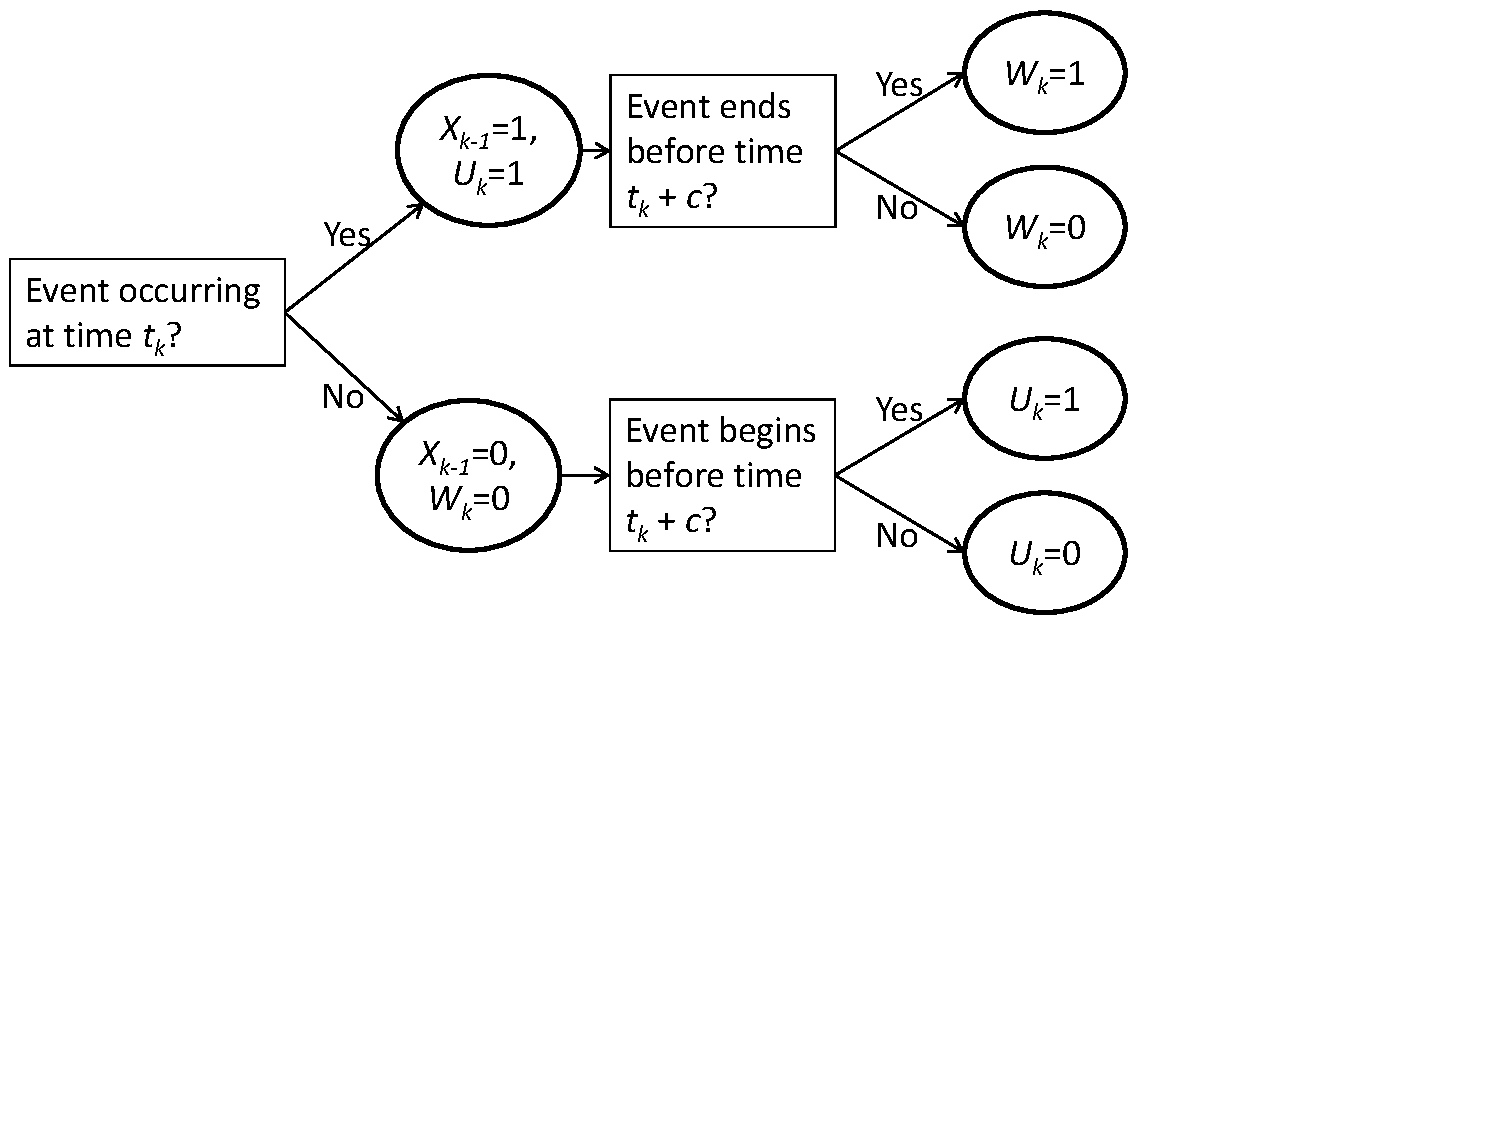
\includegraphics[clip=true, trim= 0 240 150 00, width=0.8\linewidth]{AIR_flowchart.pdf}
\caption{Procedure for combining MTS and interval recording}
\label{fig:questions}
\end{figure}  

The AIR procedure requires only marginally more effort on the part of the observer than an interval recording method used alone. 
One measure of effort is the level of sustained attention required on the part of the observer. Because the sustained attention needed for interval recording also entails the attention needed for momentary time sampling, the additional effort is minimal in this respect.
Another measure of effort is the amount of data that must be recorded during the observation period. Because $W_k = 0$ is implied when $X_{k-1} = 0$ and $U_k = 1$ is implied when $X_{k-1} = 1$, AIR requires twice as much data as one of the single methods (rather than three times as much, as might be supposed). 
Thus, for a fixed interval length, simultaneous use of all three methods entails at most twice as much effort as interval recording alone. 
Furthermore, using longer time-intervals with fewer intervals per observation period would mitigate the effort required.

Under the assumptions of the Alternating Poisson Process, the data generated by the AIR system can be modeled using a discrete-time Markov Chain, from which estimates of prevalence and incidence can be obtained. 
The Markov property of the Alternating Poisson Process implies that the joint distribution of the measurements can be written as
\begin{multline}
\Pr\left(X_0=x_0,X_1=x_1,U_1 = u_1, W_1 = w_1,..., X_K=x_K, U_K = u_K, W_K = w_K \right) \\ = \Pr\left(X_0 = x_0\right) \prod_{k=1}^K \Pr\left(X_k = x_k, U_k = u_k, W_k = w_k | X_{k-1} = x_{k-1}\right). 
\end{multline}
Denote the transition probabilities $\Pr\left(X_k = b, U_k = c, W_k = d | X_{k-1} = a\right) = \pi_{a|bcd}$ and let $m_{a|bcd} = \sum_{k=1}^K I\left(X_{k-1} = a, X_k = b, U_k = c, W_k = d \right)$ for $a,b,c,d = 0,1$. 
Conditional on $X_0$, the log-likelihood of the observed AIR data is given by
\begin{equation}
\label{eq:AIR_loglik}
l_{AIR}\left(\phi,\zeta\right) = \sum_{a=0}^1 \sum_{b=0}^1 \sum_{c=0}^1 \sum_{d=0}^1 m_{a|bcd} \log \pi_{a|bcd}
\end{equation}
where
\begin{align*}
\pi_{0|000} &= \left[1 - p_0(d)\right]\exp\left(\frac{- \zeta c}{1 - \phi}\right) \\
\pi_{0|010} &= 1 - p_0(c + d) - \left[1 - p_0(d)\right]\exp\left(\frac{- \zeta c}{1 - \phi}\right) \\
\pi_{0|100} &= p_0(d)\exp\left(\frac{- \zeta c}{1 - \phi}\right) \\
\pi_{0|110} &= p_0(c + d) - p_0(d) \exp\left(\frac{- \zeta c}{1 - \phi}\right) \\
\pi_{1|010} &= 1 - p_1(c + d) - \left[1 - p_1(d)\right]\exp\left(\frac{- \zeta c}{\phi}\right) \\
\pi_{1|011} &= \left[1 - p_1(d)\right]\exp\left(\frac{- \zeta c}{\phi}\right) \\
\pi_{1|110} &= p_1(c + d) - p_1(d) \exp\left(\frac{- \zeta c}{\phi}\right) \\
\pi_{1|111} &= p_1(d)\exp\left(\frac{- \zeta c}{\phi}\right)
\end{align*}
and the remaining transition probabilities are all equal to zero. 
See Appendix \ref{app:AIR_derivation} for the derivation of these quantities. 
As with PIR data, the MLEs $\hat\phi_{AIR}, \hat\zeta_{AIR}$ are obtained by maximizing $l_{AIR}$ using the Nelder-Mead algorithm. 

\section{Intermittent transition recording}
\label{sec:ITR}

\section{Discussion}
\label{sec:discussion}

In this paper, we have considered how to estimate the prevalence and incidence of a state behavior from data collected using conventional intermittent observation recording systems, including momentary time sampling, partial interval recording, and whole interval recording. Following earlier work by \citet{Brown1977estimation} on MTS, we used an Alternating Poisson Process to model the behavior stream as perceived by the observer, from which models for PIR and WIR data can be derived. For estimating the model parameters, simulation evidence indicated that penalized likelihood methods with generic, weak priors generally outperformed maximum likelihood methods--often dramatically so. For PIR data, penalized likelihood estimates of prevalence provided much more accurate estimates than the naiv\"e summary proportion, which is currently widely used.

We have also described a novel recording procedure, augmented interval recording, that involves combining MTS, PIR, and WIR. For a given period of observation, and using intervals twice the length of other procedures, AIR provides estimates of prevalence that are only slightly less accurate than estimates based on MTS, while also providing estimates of incidence that are substantially more accurate than estimates based on any other procedure. Of course, at present these advantages are only theoretical. To determine whether AIR offers any advantage in practice, its feasibility in real-life research contexts will need to be assessed.  

Across all of the recording procedures that we have considered, the foremost limitation of the proposed models and estimation techniques is the strength of the assumptions entailed by the Alternating Poisson Process model for the behavior stream. The model posits that the individual episodes of behavior and spans of time in between episodes are exponentially distributed. Whether these distributional assumptions are reasonable--and for what classes of behavior--is an important question requiring further empirical research. Addressing it will likely require measuring the behavior of a large sample of participants using intensive, continuous recording techniques. 
Another related avenue of further research is to examine the extent to which the proposed estimation techniques are robust to violations of the distributional assumptions (e.g., assuming that event durations follow a gamma distribution that has lower variance than the exponential). 
It may well be that the robustness of the PLEs depends on which system is used to record the data, and whether prevalence or incidence is of primary interest.

Several other limitations of these models should also be acknowledged. Our approach has treated the recording procedures themselves as essentially mechanical procedures that can be applied without human error, yet in practice the procedures are not perfectly reliable--as evidenced by the high level of inter-rater variability in the \citet{Johnson2014} data. Arguably, the model we have considered could be interpretted as implicitly accommodating rater error by allowing that the Alternating Poisson Process describes the observer's \textit{perception} of the behavior stream, rather than the true behavior stream. However, a more explicit approach to accounting for human error in the recording process would be more useful. How to extend the model in this respect remains an open question for further research.

Another limitation of the models is that they are limited to describing measurement error from a single observation session. In practice, systematic behavioral observation data is often collected on a single participant across many sessions (as in a single-case study) or across many participants (as in a between-subjects experiment). In either setting, it would be useful to embed the measurement model that we have proposed in a generalized linear modeling framework, which could be used to describe changes in prevalence and incidence across time, or in a random-effects framework, which could be used to describe between-subjects variation in the characteristics of behavior streams.

Despite these limitations, the models and estimation methods that we have proposed are nonetheless useful. For MTS data, penalized likelihood provides a means to estimate incidence as well as to assess the extent of measurement error in the estimate of prevalence. For PIR data, the penalized likelihood estimates of prevalence represent an improvement over the current standard approach, which is to simply ignore the bias in the summary proportion. Though not the focus of the present paper, the models that we have described can also be applied to develop better psychometric guidance for behavioral observation data. Through further mathematical analysis or though computer simulation, the models that we have presented could be used to study how choices regarding recording procedures, interval lengths, rest times, and observation session lengths influence the precision of behavioral measurements. Guidance regarding these aspects of study design would be useful to applied researchers designing single-case experiments or between-subjects trials.

\bibliographystyle{apacite}
\bibliography{\bibfile}
 
\appendix

\section{Derivation of PIR model}
\label{app:PIR_derivation}

The joint distribution of PIR observations depends on the conditional probabilities $\psi_k = \Pr\left[ Z(t_k) = 1 \left| U_1,...,U_{k-1}\right.\right]$. 
This appendix provides a derivation of Expression (\ref{eq:psi_k}) in terms of the parameters of the Alternating Poisson Process. The derivation will make use of the following lemma.

\begin{lemma}
\label{lemma1}
The conditional probabilities of $Z(t_k) = 1, U_{k-1} = 1$ given $Z(t_{k-1})$ are:
\begin{align*}
\Pr\left(Z(t_k) = 1, U_{k-1} = 1 \left| Z(t_{k-1}) = 1 \right.\right) &= p_1(c + d) \\
\Pr\left(Z(t_k) = 1, U_{k-1} = 1 \left| Z(t_{k-1}) = 0 \right.\right) &= p_0(c + d) - p_0(d) \exp\left(\frac{- \zeta c}{1 - \phi}\right).
\end{align*}
\end{lemma}

\begin{proof}
Observe that \[
\Pr\left(Z(t_k) = 1, U_{k-1} = 1 \left| Z(t_{k-1}) = 1 \right.\right) = \Pr\left(Z(t_k) = 1 \left| Z(t_{k-1}) = 1 \right.\right) = p_1(c + d) \]
and \begin{align*}
\Pr &\left(Z(t_k) = 1, U_{k-1} = 1 \left| Z(t_{k-1}) = 0 \right.\right) \\
& \qquad \qquad = \int_0^c\frac{p_1(c - t) \zeta}{(1 - \phi)}\exp\left(\frac{-\zeta t}{1 - \phi}\right) dt \\
& \qquad \qquad  = \phi \left[ 1 - \exp\left(\frac{- \zeta (c + d)}{\phi(1 - \phi)}\right) - \exp\left(\frac{- \zeta c}{1 - \phi}\right) + \exp\left(\frac{- \zeta (\phi c + d)}{\phi(1 - \phi)}\right)\right] \\
& \qquad \qquad = p_0(c + d) - p_0(d) \exp\left(\frac{- \zeta c}{1 - \phi}\right).
\end{align*}
\end{proof}

Turning to the derivation of $\psi_k$, begin by noting that $U_{k-1} = 0$ implies that $Z(t_k + c) = 0$. 
It follows from the Markov property that 
\begin{multline*}
\Pr\left(Z(t_k) = 1 \left| U_1 = u_1,...,U_{k-2} = u_{k-2}, U_{k-1} = 0 \right.\right) \\ 
= \Pr\left(Z(t_k) = 1 \left| Z(t_{k-1} + c) = 0 \right.\right) = p_0(d).
\end{multline*}
Next, Lemma \ref{lemma1} implies that \begin{multline*}
\Pr\left(Z(t_k) = 1, U_{k-1} = 1 \left| U_1,...,U_{k-2} \right.\right) \\
= \psi_{k-1} p_1(c + d) + (1 - \psi_{k-1}) \left[p_0(c + d) - p_0(d) \exp\left(\frac{- \zeta c}{1 - \phi}\right)\right].
\end{multline*}
It therefore follows that 
\begin{multline*}
\Pr\left(Z(t_k) = 1 \left| U_1 = u_1,...,U_{k-2} = u_{k-2}, U_{k-1} = 1 \right.\right) \\
= \frac{\psi_{k-1} p_1(c + d) + (1 - \psi_{k-1}) \left[p_0(c + d) - p_0(d) \exp\left(\frac{- \zeta c}{1 - \phi}\right)\right]}{1 - (1 - \psi_{k-1})\exp\left( \frac{-\zeta c}{1 - \phi}\right)}.
\end{multline*}
Thus, $\psi_k$ can be written as a function of $\psi_{k-1}$ and $u_{k-1}$, as given in (\ref{eq:psi_k}).

\section{Derivation of AIR model}
\label{app:AIR_derivation}

This appendix provides a derivation of the transition probabilities for the AIR model in terms of the parameters of the Alternating Poisson Process. Begin by noting that, by the definitions of the recording procedures, $X_{k-1} = 0$ implies that $W_k = 0$ and $X_{k-1} = 1$ implies that $U_k = 1$. It follows that $\pi_{0|bc1} = 0$ for $b,c = 0,1$ and $\pi_{1|b0d} = 0$ for $b,d=0,1$. Derivation of the other transition probabilities will make use of the following lemma. (The proof follow the same logic as in Lemma \ref{lemma1}, and is therefore omitted.)

\begin{lemma}
\label{lemma2}
The conditional probability of $Z(t_k) = 1, W_{k-1} = 0$ given that $Z(t_{k-1}) = 1$ is
\[
\Pr\left(Z(t_k) = 1, W_{k-1} = 0 \left| Z(t_{k-1}) = 1 \right.\right) = p_1(c + d) - p_1(d) \exp\left(\frac{- \zeta c}{\phi}\right). \]
\end{lemma}

Turning to the eight remaining transition probabilities, note that
\begin{align*}
\pi_{0|100} &= \Pr\left(X_k = 1, U_k = 0 | X_{k-1} = 0\right) \\
&= \Pr\left(X_k = 1 | Z(t_k + c) = 0\right) \Pr\left(U_k = 0 | X_{k-1} = 0\right) \\
&= p_0(d)\exp\left(\frac{- \zeta c}{1 - \phi}\right).
\end{align*}
Similarly,
\begin{align*}
\pi_{0|000} &= \Pr\left(X_k = 0, U_k = 0 | X_{k-1} = 0\right) = \left[1 - p_0(d)\right]\exp\left(\frac{- \zeta c}{1 - \phi}\right) \\
\pi_{1|111} &= \Pr\left(X_k = 1, W_k = 1 | X_{k-1} = 1\right) = p_1(d)\exp\left(\frac{- \zeta c}{\phi}\right) \\
\pi_{1|011} &= \Pr\left(X_k = 0, W_k = 1 | X_{k-1} = 1\right) = \left[1 - p_1(d)\right]\exp\left(\frac{- \zeta c}{\phi}\right).
\end{align*}
Next, it follows from Lemmas \ref{lemma1} and \ref{lemma2} that
\begin{align*}
\pi_{0|110} &= \Pr\left(X_k = 1, U_k = 1 | X_{k-1} = 0\right) = p_0(c + d) - p_0(d) \exp\left(\frac{- \zeta c}{1 - \phi}\right) \\
\pi_{1|110} &= \Pr\left(X_k = 1, W_k = 0 | X_{k-1} = 1\right) = p_1(c + d) - p_1(d) \exp\left(\frac{- \zeta c}{\phi}\right).
\end{align*}
The two remaining transition probabilities can be obtained by subtraction:
\begin{align*}
\pi_{0|010} &= 1 - \pi_{0|000} - \pi_{0|100} - \pi_{0|110} = 1 - p_0(c + d) - \left[1 - p_0(d)\right]\exp\left(\frac{- \zeta c}{1 - \phi}\right) \\
\pi_{1|010} &= 1 - \pi_{1|011} - \pi_{1|110} - \pi_{1|111} = 1 - p_1(c + d) - \left[1 - p_1(d)\right]\exp\left(\frac{- \zeta c}{\phi}\right).
\end{align*}
\end{document}
